\documentclass[12pt,twoside]{report}
\pagenumbering{roman}

\usepackage{graphicx}
\usepackage{subcaption}
\usepackage[utf8]{inputenc}
\usepackage[german]{babel}
% for units
\usepackage{siunitx}

\usepackage{hyperref}
\hypersetup{
  colorlinks=true,
  linkcolor=blue,
  filecolor=magenta,      
  urlcolor=cyan,
}

\urlstyle{same}

\begin{document}
\begin{titlepage}
    \begin{center}
        \vspace*{1cm}
            
        \Huge
        \textbf{Lernportfolio}

        \vspace{1.5cm}
            
        \normalsize
        \textbf{Pierre Dahmani pd1528s 3215892\\
        Jens Peter Dennigmann jd8389s 3190025 \\
        Leonhard Kipp lk2149s 3188047\\}
            
        \vfill
            
        EES Buggy-Projekt 
        \vspace{0.8cm}
            
        %% TODO Add title pic
        %% \includegraphics[width=0.4\textwidth]{university}
        \pagebreak
    \end{center}
\end{titlepage}

% TODO Inhaltsverzeichnis

\begin{section}{Aufbau des Buggy}

\begin{figure}[h!]
  \centering
  \captionsetup[subfigure]{labelformat=empty}
  \begin{subfigure}{0.45\linewidth}
    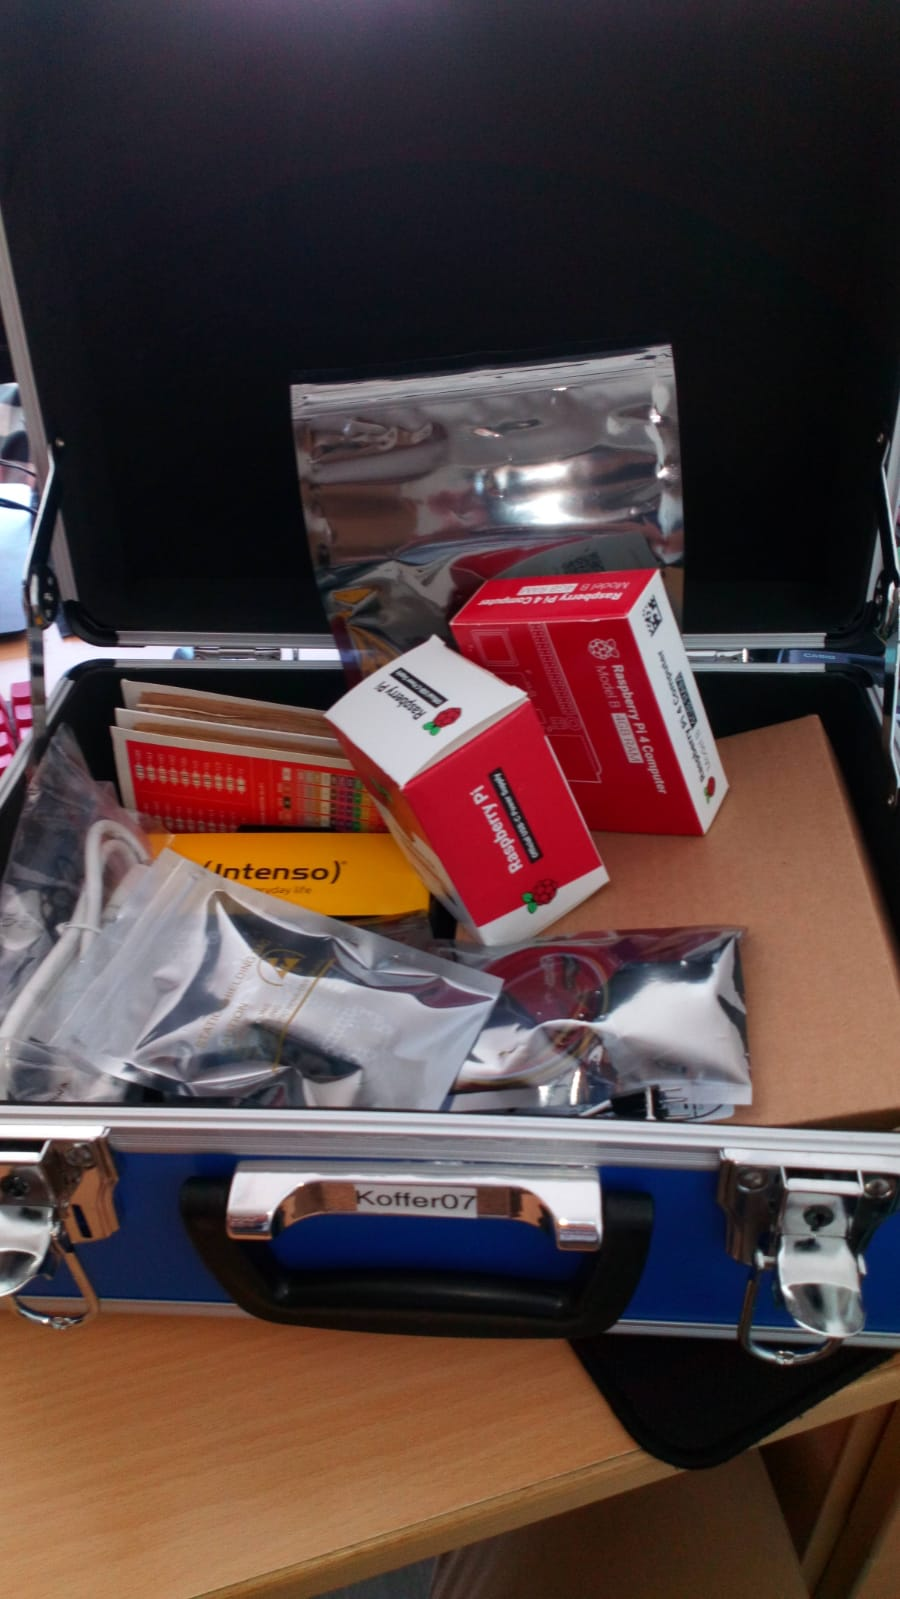
\includegraphics[width=\linewidth]{lernportfolio_assets/Buggy_Koffer.jpeg}
    \caption{Der Buggy vor dem Aufbau.}
  \end{subfigure}
  \begin{subfigure}{0.45\linewidth}
    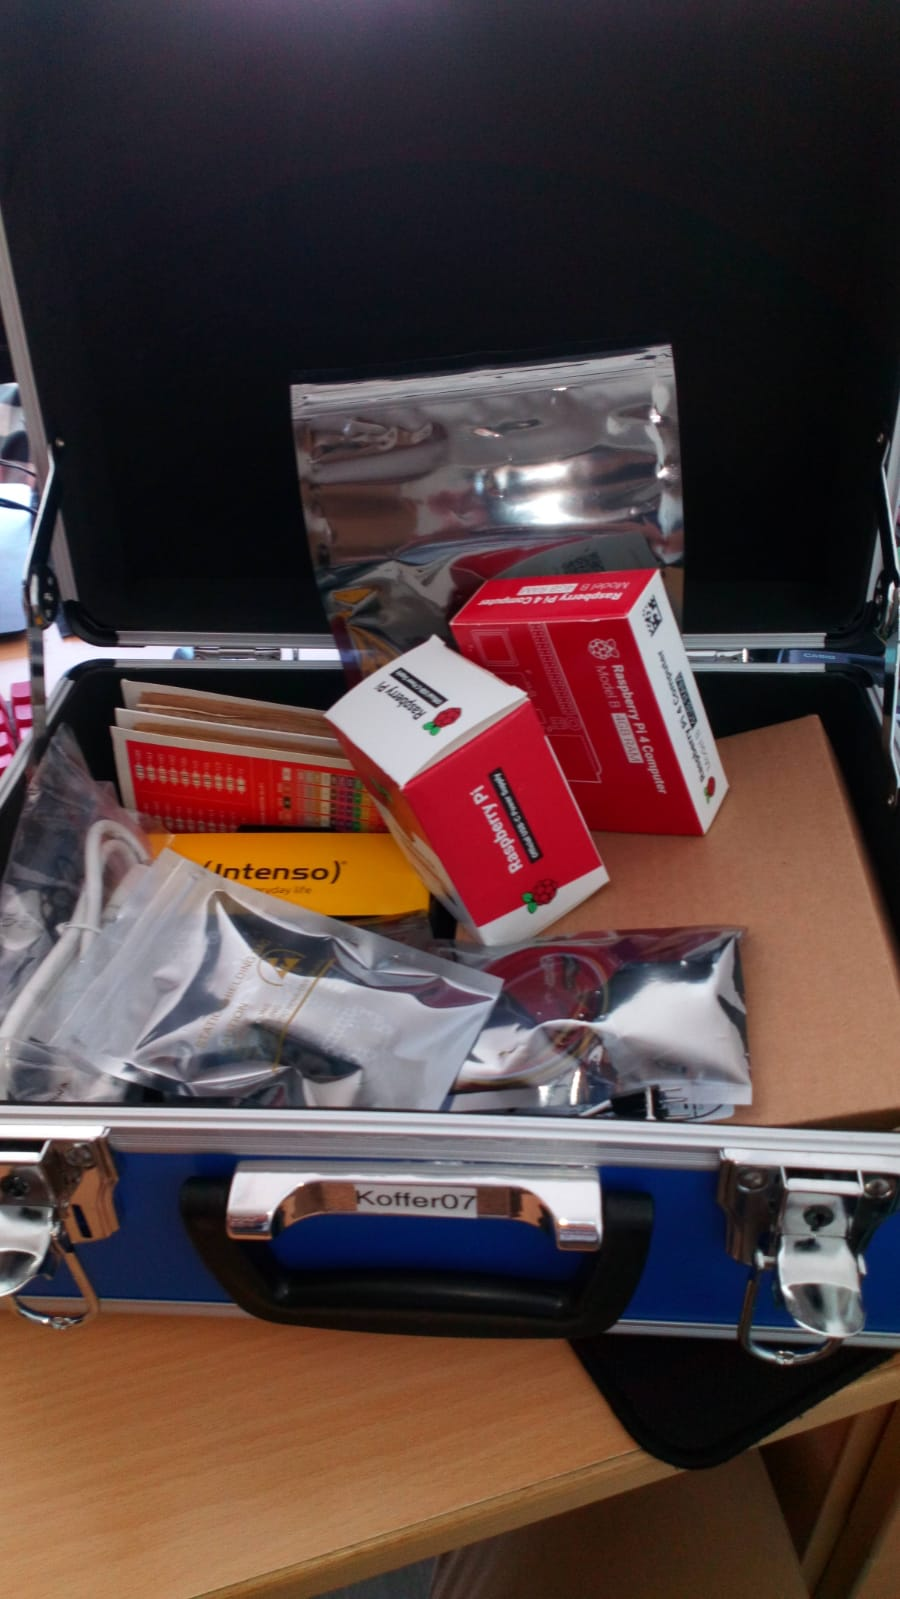
\includegraphics[width=\linewidth]{lernportfolio_assets/Buggy_Koffer.jpeg}
    \caption{Und danach.}
  \end{subfigure}
\end{figure}

Der Buggy wurde vor der Herausgabe des Arbeitsauftrages zusammengebaut. Zwischenschritte sind daher nicht bildlich festgehalten. 

Der Zusammenbau des Buggies verlief problemlos. Der Text ist insgesamt verständlich geschrieben und war eine große Unterstützung.

% Wollen wir das aufnehmen?
% Im Text ist der Genetiv von ``der Buggy'' durchgehend ``des Buggies''. Mit Verweis
% auf \url{https://www.duden.de/rechtschreibung/Buggy} ist der korrekte - und
% kontraintuitive - Genetiv ``des Buggys''.
In den meisten Bildern (außer auf Seite IV) ist der Buggy mit roter Platte gezeigt, wenngleich die Anleitung hier den weißen Winkel vorsieht. Eine Anmerkung, dass der Buggy im Folgendem mit roter Platte statt Winkel gezeigt wird, hätte eine kurze Verwirrung meinerseits verhindert.

Als Ubuntu-Nutzer muss man keine zusätzliche Software installieren um eine SSH-Verbindung herzustellen. Eine Ergänzung, dass \href{https://invisible-island.net/xterm/}{XTerm} eine Empfehlung an die Windows-Nutzer ist, wäre daher angebracht. Bei dieser Bemerkung wird davon ausgegangen, dass mit XTerm an dieser Stelle \href{https://mobaxterm.mobatek.net/}{MobaXterm} gemeint ist und nicht der Terminal Emulator XTerm. 

Für den kompletten Zusammenbau wurden insgesamt 1 Stunden benötigt. Die meiste Zeit nahm die SSH-Verbindung in Anspruch.

Weil der Buggy schon vor Herausgabe des Arbeitsauftrages und während der anhaltenden Corona Phase abgeholt worden ist, wurde der Buggy von einer Person aufgebaut. Im Nachhinein haben wir uns trotzdem Gedanken dazu gemacht, wie wir den Aufbau am besten hätten aufteilen können. Wir sind zu dem Ergebnis gekommen, dass jede Person einen Teil des Buggys aufbauen sollte. Konkret hätte sich einer um das Kugellager und die Motoren gekümmert. Einer um die Abstandhalter und das Anbringen der Plastikplatte und des Raspberry Pi. Der letzte um das Anbringen des Motorhats und um das Anschließen und Fixieren der Powerbank.

\end{section}

\begin{section}{Motorensteuerung}

    TODO Motorensteuerung recap

    TODO Video einfügen von der Rechteckfahrt objects/rectangle.mp4

\end{section}

\begin{section}{Ultraschallsteuerung}
    \begin{subsection}{Recherche zum Ultraschallsensor}
        Quellen:
        http://blog404de.github.io/RasPiUltraschallEntfernungsmesser/
        https://www.einplatinencomputer.com/raspberry-pi-ultraschallsensor-hc-sr04-ansteuern-entfernung-messen/
        https://tutorials-raspberrypi.de/entfernung-messen-mit-ultraschallsensor-hc-sr04/
    \end{subsection}
    \begin{subsection}{Aufbau}
        % \iffalse
        %     TODO: why does the picture always take a whole page and not fit inside the page?
        % \fi
        \begin{figure}[h!]
              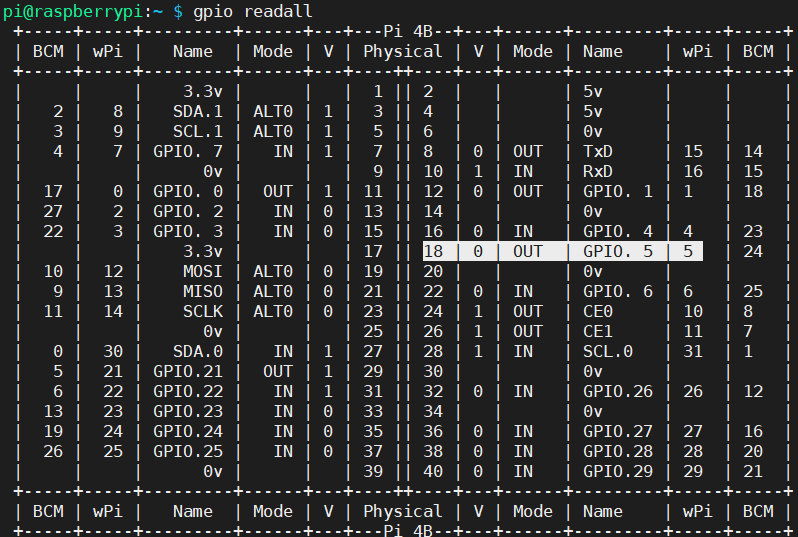
\includegraphics[width=\linewidth]{lernportfolio_assets/GPIO_Pins}
              \caption{Pin Mapping WiringPi Motorhat}
              \label{fig:boat1}
        \end{figure}
        Der Ultraschallsensor HC-SR04 hat einen Vcc, einen Gnd, einen Trigger und einen Echo Anschluss.
        Der Ultraschallsensor benötigt eine Versorungsspannung von 5 Volt , die können wir direkt vom Motorhead nutzen.
        Der Trigger wird durch den GPIO Pin 5 auf dem Motorhead und damit dem Pin 21 der wiringPi Bibliothek gesetzt.
        Das Echo Signal würde eine Spannung von 5V betragen. Da der Pi jedoch nur eine Spannung von 3,3V verträgt, muss man hier einen Vorwiderstand von 330$\Omega$ verwenden. Zusätzlich wird ein Pull-Down Widerstand in Höhe von 470$\Omega$ angeschlossen um einen floating state zu verhindern und den Pin gegen Ground zu ziehen.
        Der Gnd wird direkt an den Gnd vom Motorhat angeschlossen.

        \begin{figure}
            \centering
            \begin{minipage}{0.45\textwidth}
                \centering
                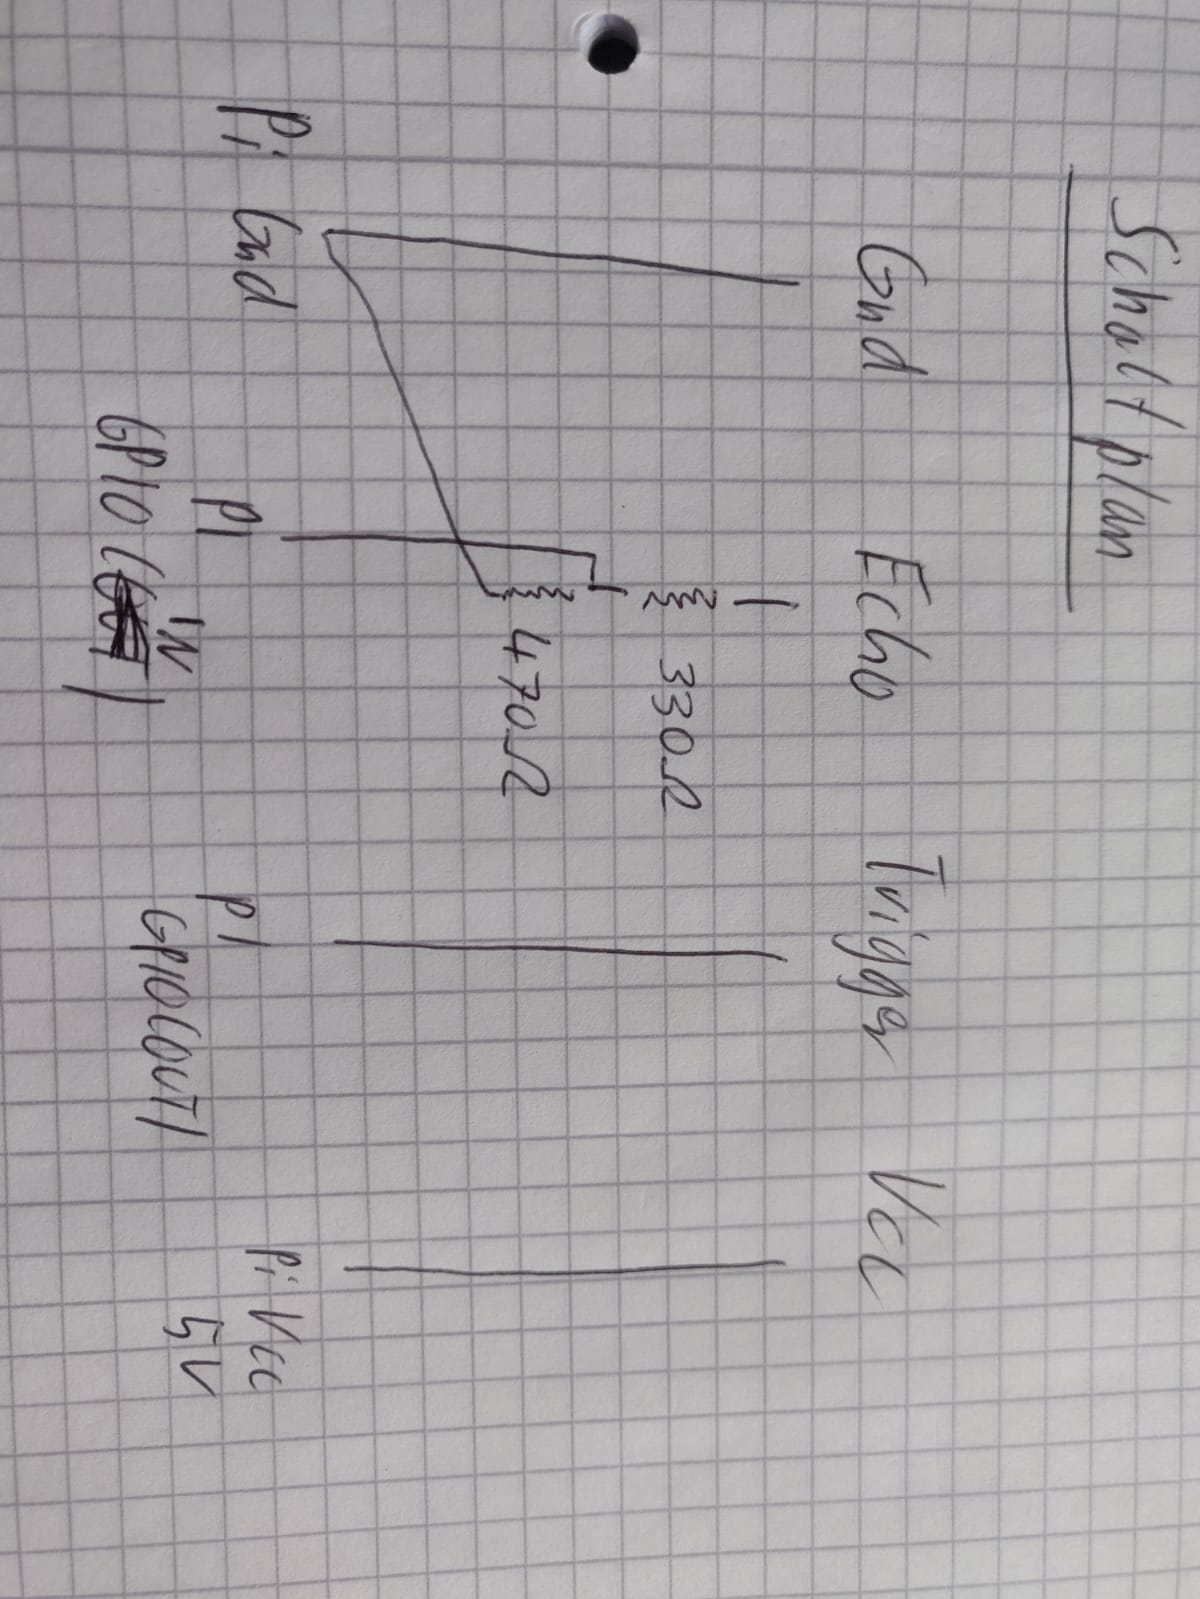
\includegraphics[width=0.9\textwidth]{lernportfolio_assets/Schaltplan_Ultraschallsensor1} % first figure itself
                \caption{Auf Papier}
            \end{minipage}
            \hfill
            \begin{minipage}{0.45\textwidth}
                \centering
                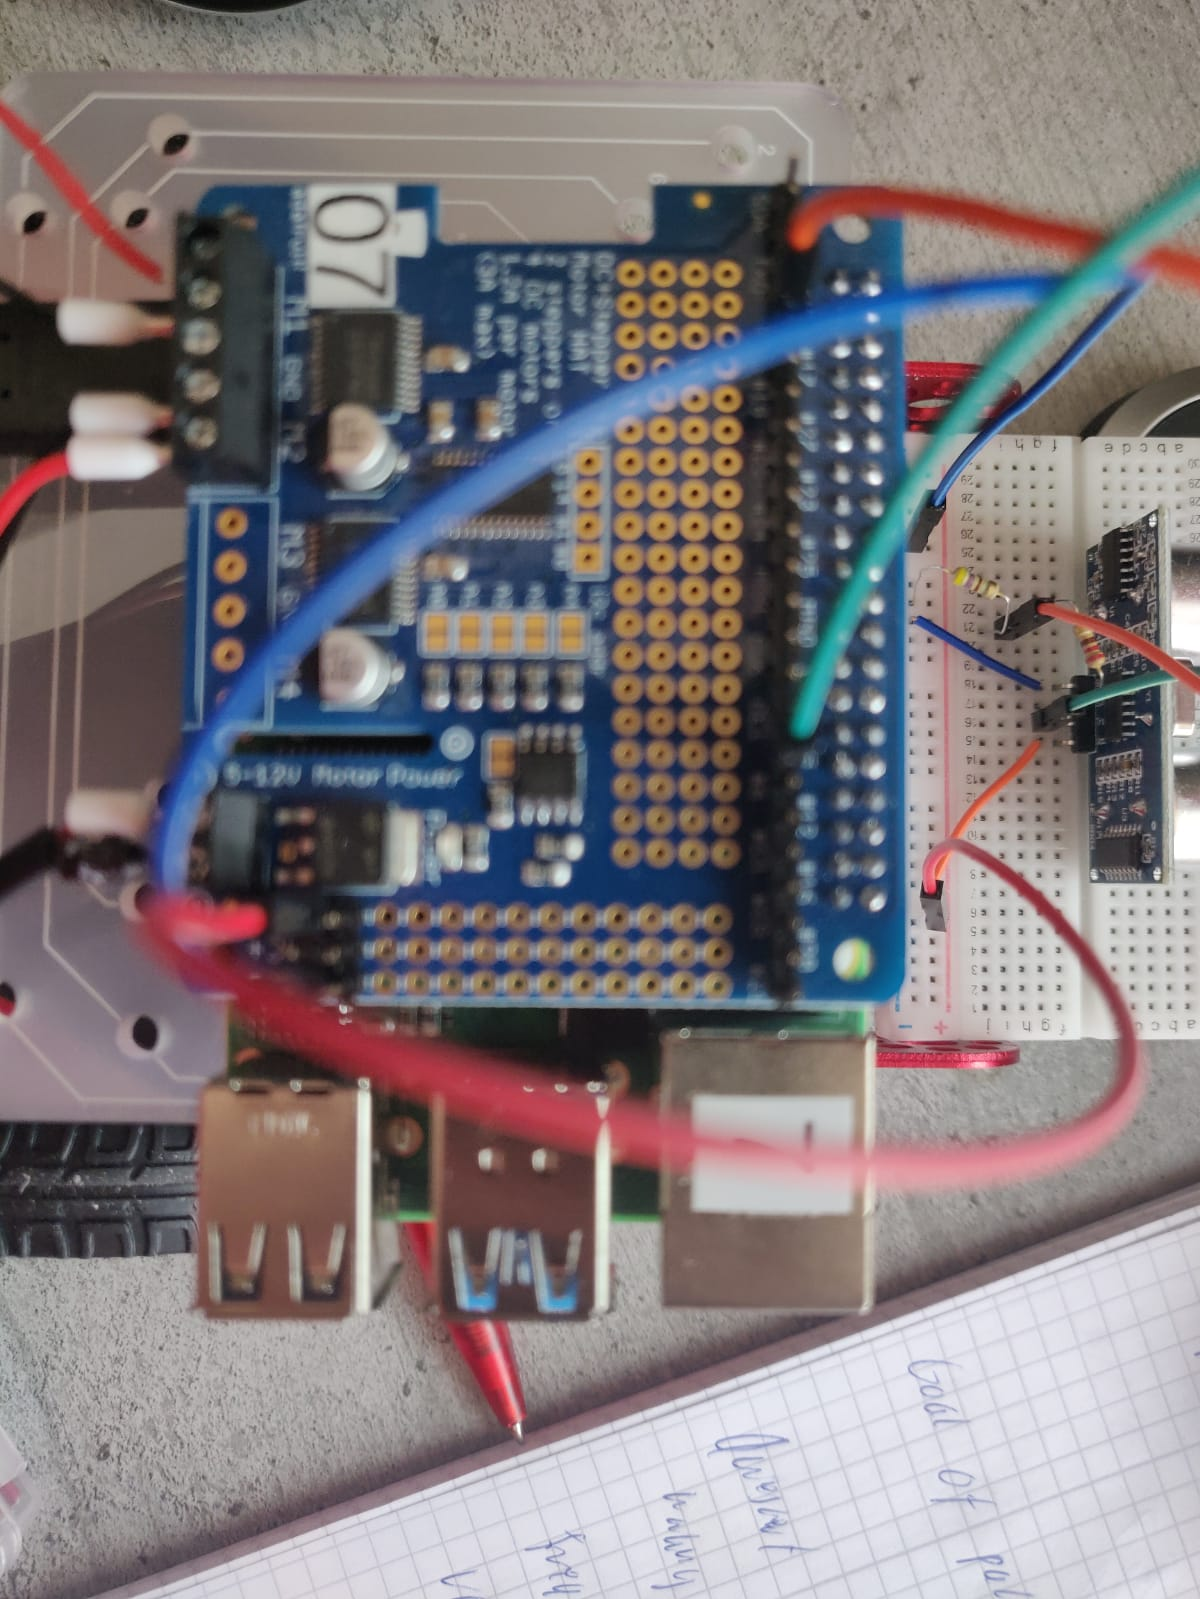
\includegraphics[width=0.9\textwidth]{lernportfolio_assets/Schaltplan_Ultraschallsensor2} % second figure itself
                \caption{Auf Papier}
            \end{minipage}
        \end{figure}
    \end{subsection}
    \begin{subsection}{Distanzberechnung}
        Die Distanz wird durch den Ultraschallsensor berechnet indem durch den Trigger ein Signal losschickt und die Zeit misst, die das Signal braucht um am Echo anzukommen. 
        Distanz (in \si\cm)= \( \frac{Signalzeit}{2} \) \si\second $ \cdot $ 34350 \( \frac{\si\cm}{\si\second} \)
    \end{subsection}

    \begin{subsection}{Bewertung der Zuverlässigkeit der Entfernungsmessung}
      Die Entfernungsmessung funktioniert für solide Objekte in einer Reichweite
      von 5 bis 100 cm zuverlässig. Für weniger soliden Objekten, wie z.B. einer
      Pappierbox, hat der Sensor den Tests Probleme
      gehabt, die Entfernung richtig einzuschätzen. Oftmals kam es hierbei zu keinen Rückmeldungen an den Echo-Pin. Dieses
      Problem wurde durch ein Zeitlimit beim Warten auf den Echo-Pin gelöst.
      Die relativ hohe Varianz zwischen einzelnen Messungen bei gleicher Distanz zum Objekt
      wird durch mehrmaliges Messen und ermitteln des Durchschnittes abgefangen.
    \end{subsection}
    \begin{subsection}{Bewertung der Genauigkeit}
      Die Entfernungsmessung funktioniert mit einer Standardabweichung von unter
      1,3 cm auf 100 cm genau.
      Die Rohdaten können im Anhang \ref{ultraschallsensorRohdaten} eingesehen werden.
      Im folgendem eine Zusammenfassung.
      %The table is generated by pandas
      \begin{table}[h!]
        \begin{tabular}{lrrrrrrr}
          % \toprule
          Abstand &       5cm &        10cm &        15cm &        20cm &        30cm &        50cm &       100cm \\
          % \midrule
          count &  100.000000 &  100.000000 &  100.000000 &  100.000000 &  100.000000 &  100.000000 &  100.000000 \\
          mean  &    4.668009 &    9.355380 &   13.951283 &   19.938128 &   30.418109 &   51.078758 &   99.553521 \\
          std   &    0.032030 &    0.305832 &    0.109583 &    0.060932 &    0.107799 &    0.482031 &    1.268841 \\
          min   &    4.650300 &    8.792790 &   13.804400 &   19.811500 &   30.079000 &   50.054500 &   91.353200 \\
          25\%   &    4.663265 &    9.122402 &   13.854150 &   19.880775 &   30.405600 &   50.820775 &   99.667750 \\
          50\%   &    4.664025 &    9.305280 &   13.912850 &   19.933800 &   30.450700 &   50.999200 &   99.878350 \\
          75\%   &    4.665242 &    9.658680 &   14.020900 &   19.983375 &   30.478350 &   51.518525 &   99.959425 \\
          max   &    4.979740 &    9.821430 &   14.231100 &   20.131400 &   30.566800 &   51.951700 &  100.912000 \\
          % \bottomrule
        \end{tabular}
        \caption{Zusammenfassung der Rohdaten. Alle Werte in cm.}
    \end{table}
    Aus der Tabelle geht hervor, dass der Abstand zu nahen
    Objekten (Abstand <= 20 cm) tendenziell unterschätzt wird, zu entfernteren
    Objekten hingegen geringfügig überschätzt. Eine Ausnahme bildet hier die
    Messreihe für den Abstand von 100 cm.
    
    Um den Mittelwert gibt es für alle Werte eine Standardabweichung von weniger
    als 1,3 cm. Die Messung sind daher präzise. Erwähnenswert ist, dass die
    Standardabweichung bei kleineren Distanzen sehr viel geringer ist als bei größeren.

    \begin{figure}[h!]
      \centering
      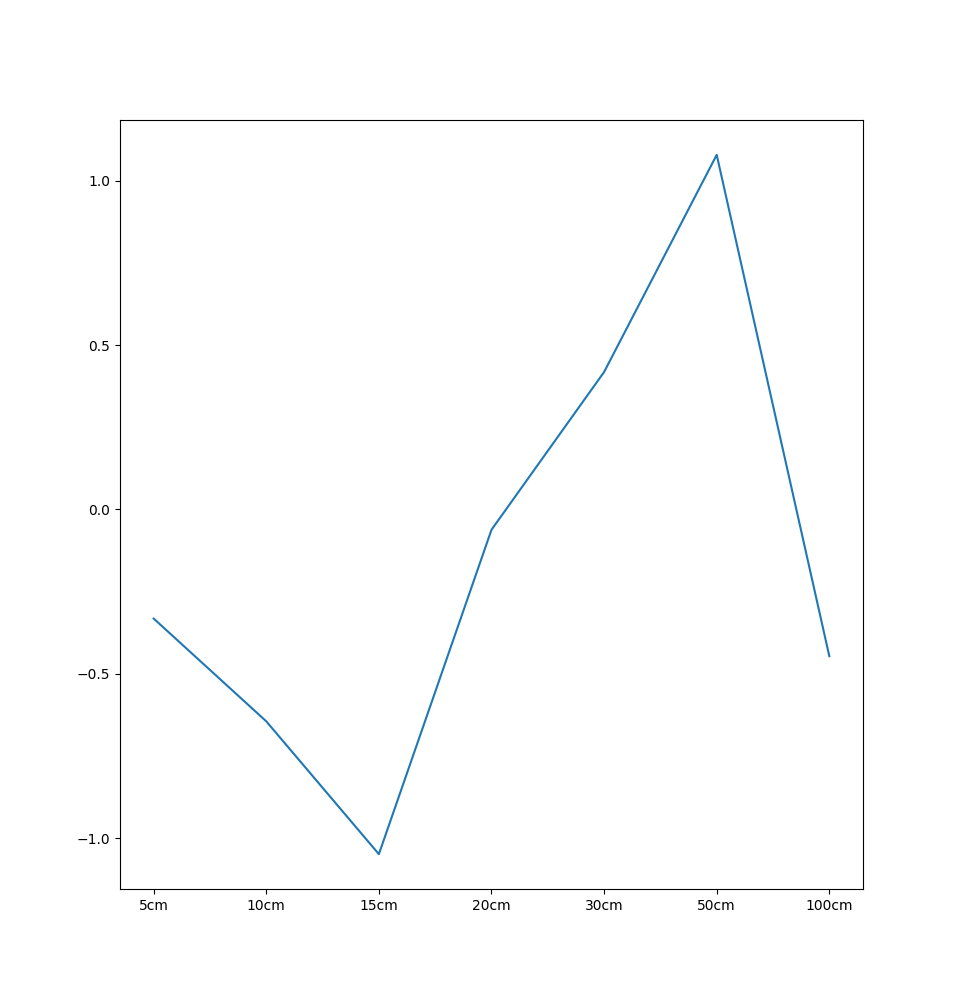
\includegraphics[width=0.5\textwidth]{test_data_ultrasonic/meanDiff.png}
      \caption{Differenz des Mittelwertes zur tatsächlichen Distanz}
    \end{figure}

  \end{subsection}

\end{section}

\begin{section}{Anhang}
  \begin{subsection}{Rohdaten Ultraschallsensor} \label{ultraschallsensorRohdaten}
    \input{test_data_ultrasonic/rohdaten.tex}
  \end{subsection}
\end{section}

\end{document}

 